\documentclass[final]{aiaa-pretty}

%\usepackage[hidelinks]{hyperref}
\usepackage{graphicx}
\usepackage{pdfpages}
\usepackage{float}
%\usepackage{caption}
\usepackage{subfigure}
\usepackage{epstopdf}
\usepackage{nomencl}%   nomenclature generation via makeindex
\usepackage{listings} % for appendix limiter .C code
% Author information
\author{ % and 
Aaron Katz\thanks{Assistant Professor, AIAA Member}, 
Shaun Harris\thanks{Undergraduate Student, AIAA Student Member},
Dalon Work\thanks{PhD Candidate, AIAA Student Member},
Oisin Tong\thanks{PHD Candidate, AIAA Student Member},
and Jon Thorne\thanks{Masters Student, AIAA Student Member} \\
\textit{Department of Mechanical and Aerospace Engineering, Utah State University, Logan, UT 84322}}
% Title
\title{Comparison of Triangular, Cell-Centered, and Node-Centered Prismatic Grid methods}

%Abstract

\makeindex
\abstract{ %
% 
This paper compares three separate algorithms for computing simple geometries and simple cases.  The cases are then analyzed and validated to compare the error.  It is concluded which method yields higher order results and therefore yielding a more accurate result.  More validation must be undertaken to back up this conclusion.
       }
\begin{document}
\maketitle



\section{Introduction}
Three separate algorithms for computing a flat plate and a bump case are shown and compared.  A triangular grid case with flux correction, a cell-centered grid case, and a node-centered grid case with flux correction are explained and a flat plate case and bump case are analyzed for each grid. The purpose of this study is to analyze the error associated with each of the three algorithms mentioned above for a few simple cases.  This abstract will present preliminary visualization of a flat plate case and a bump case.  Additionally, the node-centered prismatic grid was also run at transonic speeds with a limiter inclusion on a bump case.  The limiter computation and results are shown.  The resulting shock is shown and analyzed. 

% % % % % % % % % % % % % % % % % % % % % % % % % % % % % % % %
\section{Numerical Methods}
\subsection{Computational Approaches}
This section will outline the basic description of each of the three algorithms mentioned above.  We will not go into detail on the computation as previous papers have already done so.  We will outline the limiter inclusion computation into the node-centered grid algorithm.


\subsection{Grids}
 \subsubsection{Triangular Grid}
The triangular grid formulation uses computation discussed elsewhere \cite{Work2014}.  A section of a two dimensional flat plate is shown in figure \ref{TriG}.  

\begin{figure}[h!] %Three seperate grids used
\centering
\subfigure[Triangular grid]{
\label{TriG}
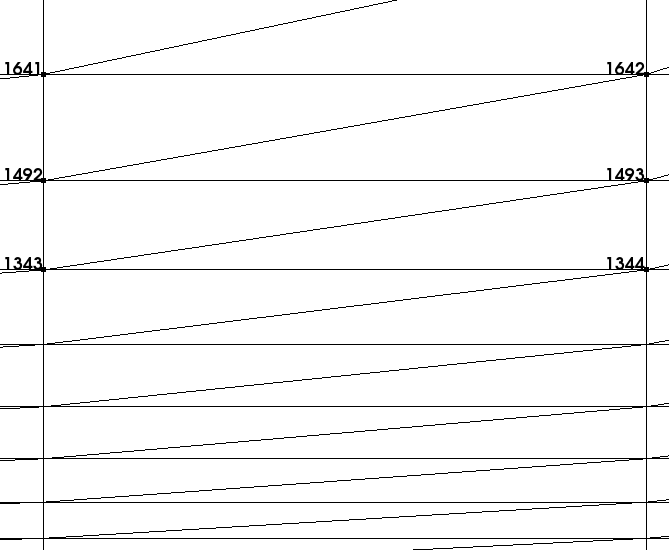
\includegraphics[width=.3\textwidth]{pics/Tri2dFC_Grid_all3.png}
}
\subfigure[Cell-centered grid]{
\label{CCG}
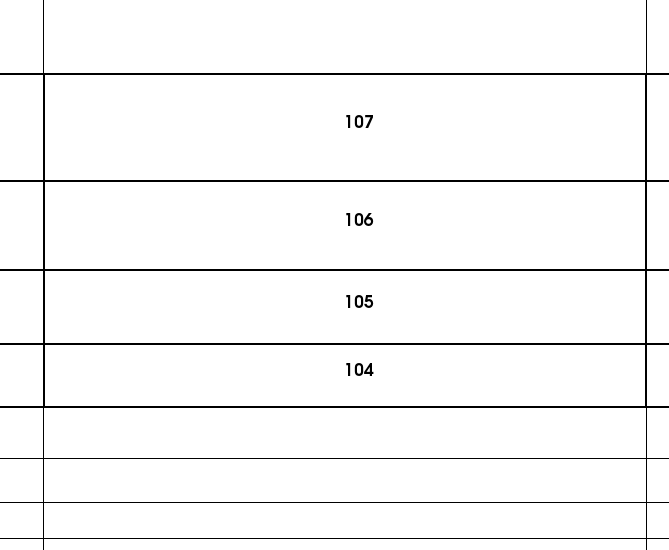
\includegraphics[width=.3\textwidth]{pics/Strand2d_Grid_all3.png}
}
\subfigure[Node-centered grid]{
\label{NCG}
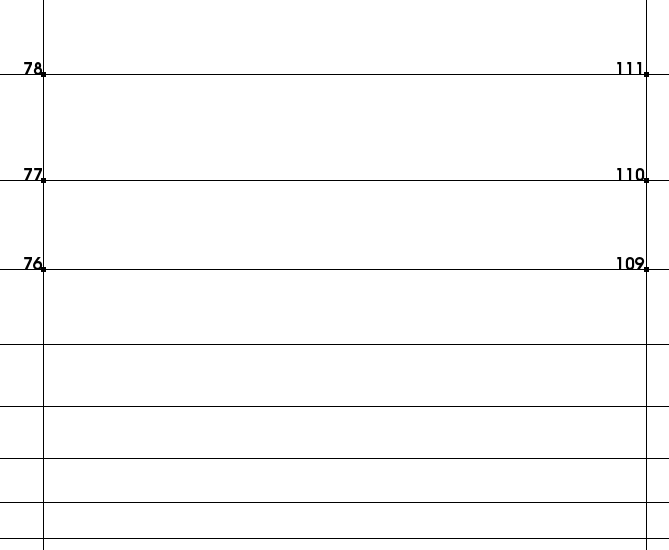
\includegraphics[width=.3\textwidth]{pics/Strand2dFC_Grid_all3.png}
}
\label{GridReps}
\caption{Visual overview of the three separate grids used in this study.  Each figure displays the identification number associated with the respective node or cell used in the calculations.}
\end{figure}




 \subsubsection{Cell-Centered Grid}
The cell-centered grid uses a prismatic approach to define the grid.  Figure \ref{CCG} shows a section of a flat plate outlined with identification numbers at the cell center points.  All numerics are computed using this grid identified at the center of each cell as referenced previously \cite{Katz2015}.  

 \subsubsection{Node-Centered Grid}
The node-centered grid uses a prismatic approach to define the grid.  Figure \ref{NCG} shows a section of a flat plate outlined with identification numbers at the node center points.  All numerics are computed using this grid identified at the center of each node as referenced previously \cite{Katz2015}.


\subsection{Limiter Inclusion}
Capturing a shock wave using a higher order method can be difficult.  The node-centered prismatic code mentioned previously \cite{Katz2015} employs a local extremum diminishing (LED) scheme.  A one dimension example of this method is shown in figure \ref{LEDstencil}.  With this scheme we can employ a limiter.  One method used to retain high order accuracy is through limited linear reconstruction, in which the left and right states for the artificial diffusion are reconstructed from surrounding nodal values to the control volume interface.  For example, at the $j + \frac{1}{2}$ interface yields  

\begin{figure}[h!]
\centering
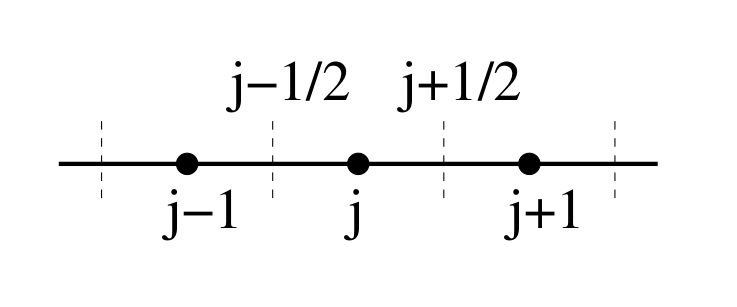
\includegraphics[width=.5\textwidth]{LED2dStencil.png}
\label{LEDstencil}
\caption{One-dimensional finite-volume stencil}
\end{figure}


\begin{equation}
Q_L = Q_j + \frac{s}{2} (x_{j+1} - x_j) \left.\frac{dQ}{dx}\right|_{j} , 
Q_R = Q_{j+1} - \frac{s}{2} (x_{j+1} - x_j)\left.\frac{dQ}{dx}\right|_{j+1}
\end{equation}

where $s$ is a limiter and the gradients of $Q$ are estimates using surrounding nodal values.
Using the reconstructed values actually renders the scheme non-LED. However, we really
only need the LED property at local extrema. The role of the limiter, $s$, is to detect these
local extrema, at which points we set $s = 0$. Otherwise, $s \approx  1$. This may be accomplished
at $j + \frac{1}{2}$ by setting

\begin{equation}
s=1 - \left| \frac{a - b}{\left|a\right| - \left|b\right|}\right|^q, 
a=Q_{j+2} - Q_{j+1},
b=Q_j - Q_{j+1}
\end{equation}

where $q$ is a positive integer taken to be three in these node-centered code cases.
If $a$ and $b$ are of opposite signs,
which would be the case at a local extremum, then $s = 0$. In smooth regions, the limiter is
nearly unity.  

In theory, this algorithm can be employed to result in a lower order approximation at the local extrema to capture a shock wave using a lower order approximation.  The rest of the domain will be approximated using a higher order scheme.  

%The code to implement this in a two dimensional scheme is shown in the appendix in section \ref{sec::APP}.


 
% % % % % % % % % % % % % % % % % % % % % % % % % % % % % % % %
\section{Preliminary Results}
We will compare the results from the flat plate and bump cases from each of the grid codes.
\subsection{Flat Plate}
Each grid ran a case of a flat plate at Mach $0.2$ and $Re = 10,000$.  The visual comparison of each of the three codes run is shown in figure \ref{FP3}.

\begin{figure}[h!]
\centering
\subfigure[Triangular grid]{
\label{TriGFP}
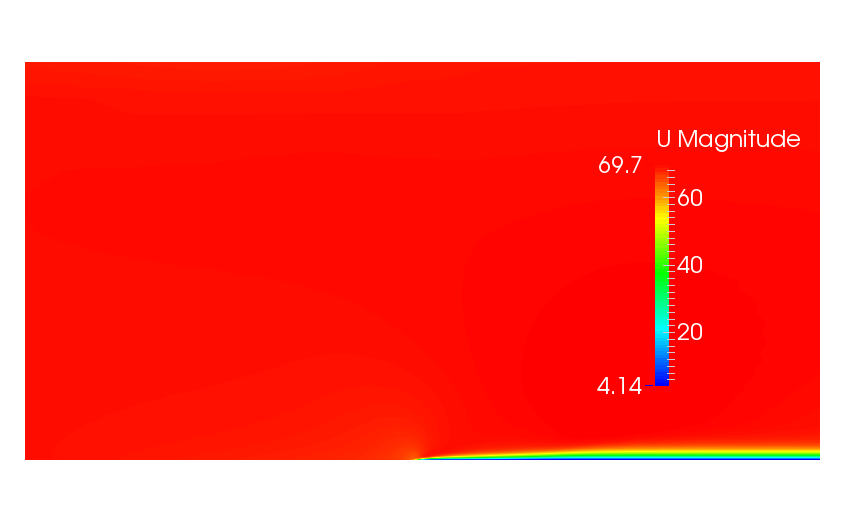
\includegraphics[width=.3\textwidth]{FlatPlate_15x/Tri2dFC_FlatPlate.png}
}
\subfigure[Cell-centered grid]{
\label{CCGFP}
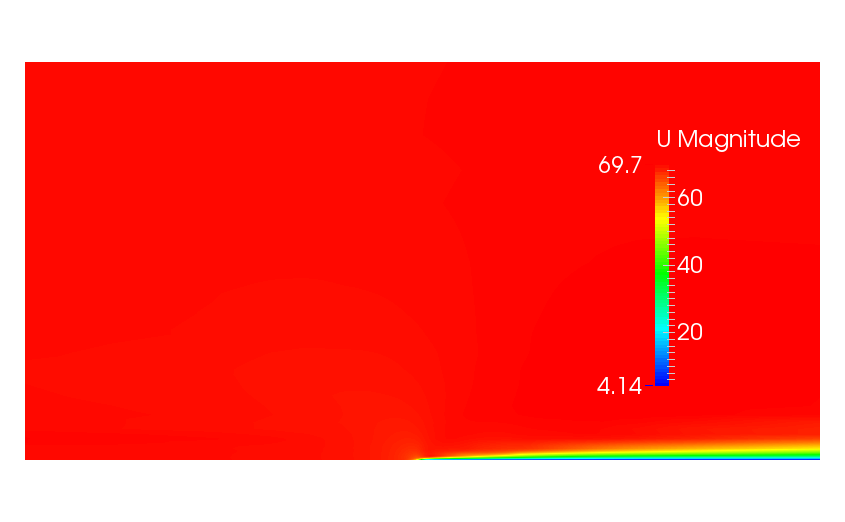
\includegraphics[width=.3\textwidth]{FlatPlate_15x/Strand2d_FlatPlate.png}
}
\subfigure[Node-centered grid]{
\label{NCGFP}
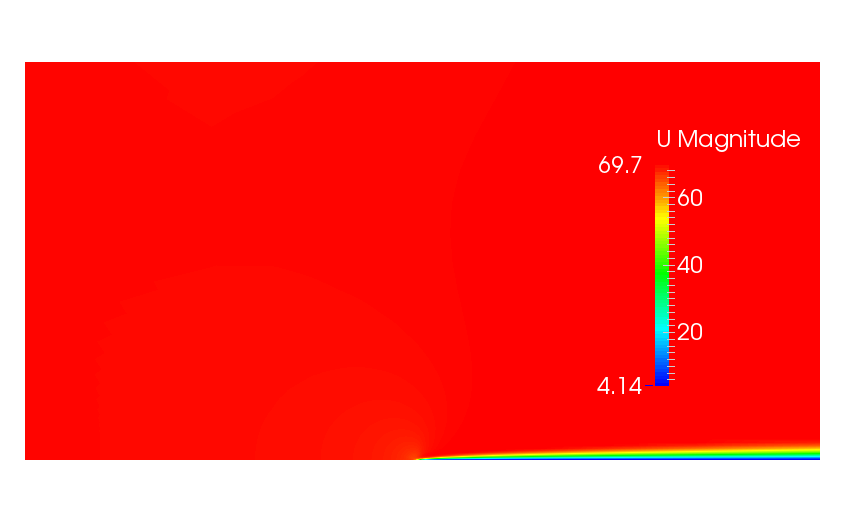
\includegraphics[width=.3\textwidth]{FlatPlate_15x/Strand2dFC_FlatPlate.png}
}\\
\subfigure[Blasius Solution comparison of all three grids.  The left axis shows the $u$ velocity direction and the right axis shows the $v$ velocity direction.]{
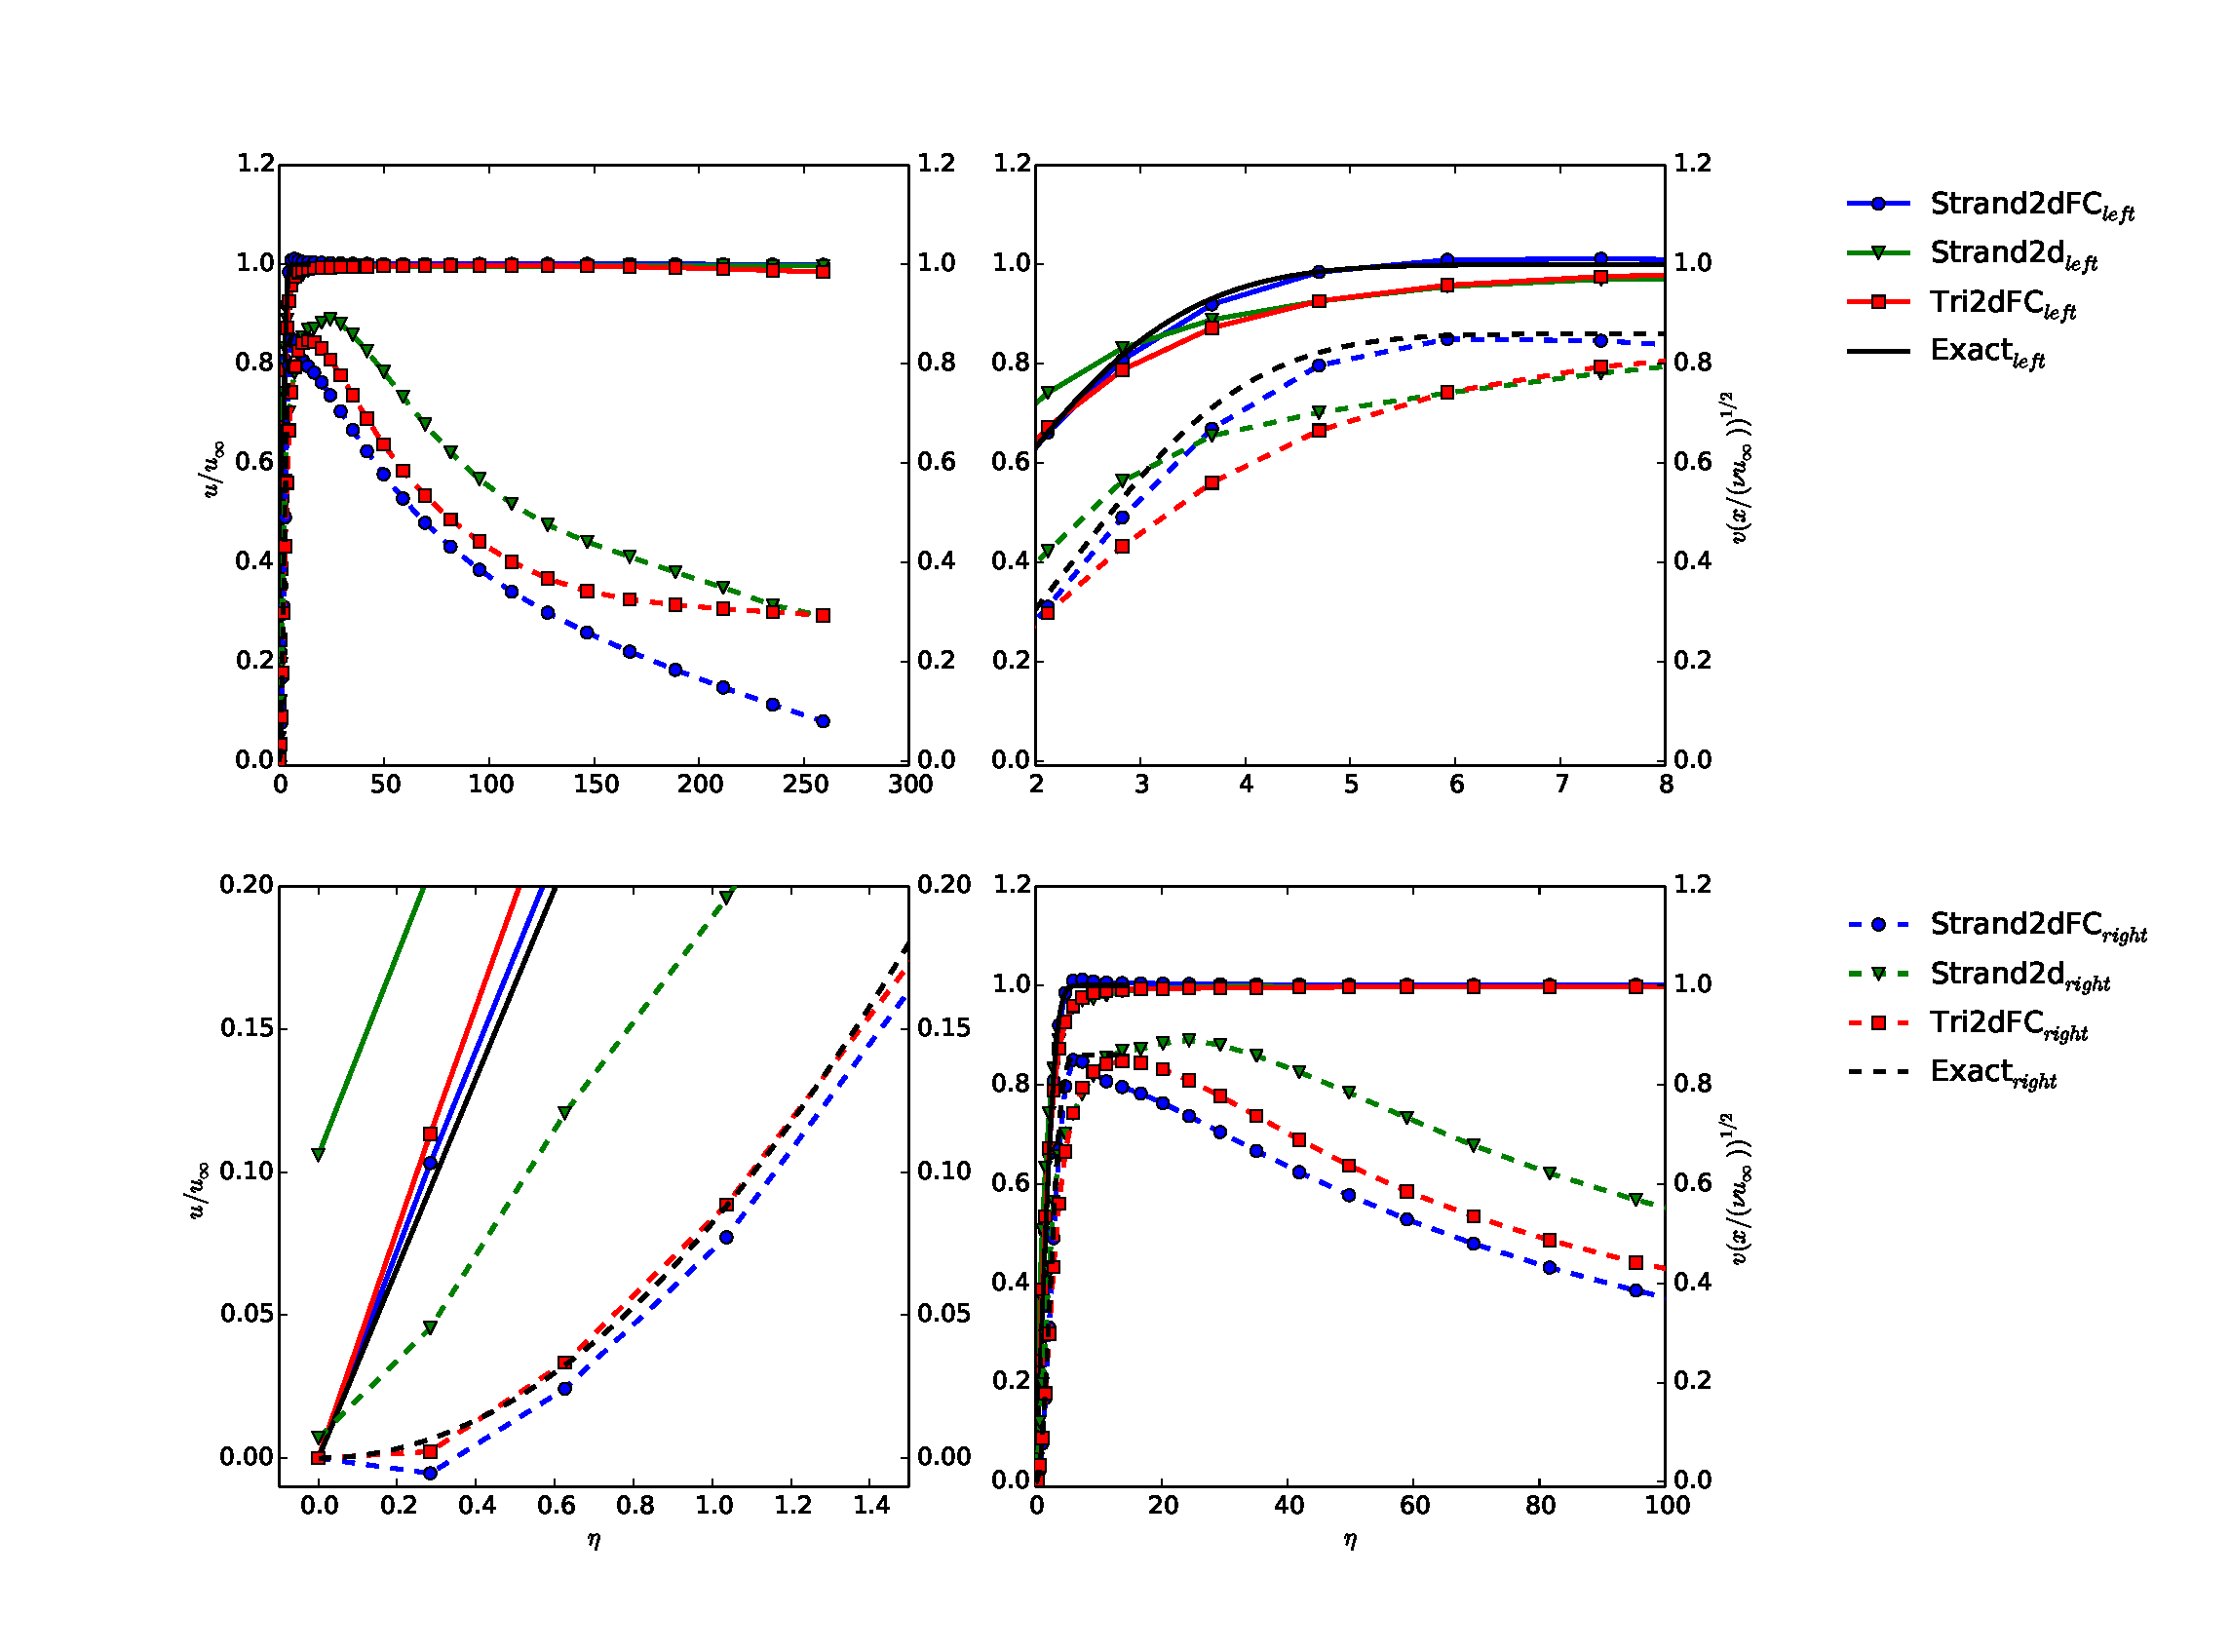
\includegraphics[width=.95\textwidth]{FlatPlate2.pdf}
\label{FPBlasius}
}
\caption{Each figure displays the flat plate case executed by each of the three algorithms associated with the respective node or cell used in the calculations. The comparison of these solutions vs the Blasius solution is also shown in four plots.}
\label{FP3}
\end{figure}

Each grid algorithm was run using a similar plate comparison of the flat plate stuff against Blasius solutions.  The plot is shown in four separate views below in figure \ref{FPBlasius}.


We can observe by visual inspection that the Strand2dFC line fits closer to the exact Blasius solution.  The Strand2dFC stands for a two-dimensional prismatic code with a flux correction.  This is also known as the previously stated node-centered prismatic grid code.  We also note that there is a significant error associated with the Strand2d code also known as the cell-centered prismatic grid code.  This error will need to be examined before the final work is submitted. 

Additionally, a study will be conducted comparing these results formally against a validation study. This will give further insight into the performance of these grid codes.

\subsection{Bump}

\subsubsection{Subsonic}
The final paper will give the results of and comparison against a validation study of a Mach $0.2$ $Re = 3$ million case.  The results will be compared and the error will give an indication for conclusive statements of the performance of the codes.
\subsubsection{Transonic Inviscid with Limiter Inclusion}
The node-centered grid algorithm was taken and run at a faster speed of Mach $0.8$.  The bump here is an inviscid boundary condition.  The resulting shock on the bump is shown in figure \ref{ITB}.

\begin{figure}[h!]
\centering
\includegraphics[width=.75\textwidth]{Scheme2_2_hiAspect.png}
\caption{Invscid transonic bump case at Mach 0.8}
\label{ITB}
\end{figure}

\begin{figure}[h!]
\centering
\includegraphics[width=.75\textwidth]{BumpPressure_2_2_Mpt8.png}
\caption{$C_p$ value along the bump at 0.8 Mach speed.  This compares the results with and without the limiter inclusion.}
\label{CP}
\end{figure}

\section{Final Paper}
The final paper research will conclude the validation error analysis of the three codes.  It will conclude analyzing the flat plate case by comparing it against a validation study.  

The final paper will include results from the subsonic case which will have an error analysis and validation study.  This, along with the flat plate cases, will yield further insight into the higher order solution given by node-centered prismatic grid algorithms.  

Additionally, the impact of the limiter will be analyzed.  Other limiter calculations will be compared and contrasted.  The impact of having high aspect ratios and geometry will also be analyzed with respect to this limiter.  

Finally, the final paper will show the value of the node-centered scheme in calculating high-order solutions for simple geometry.  This will include other studies and geometries such as a hemisphere cylinder.  

\section{Conclusions}
The preliminary results from the flat plate case has shown the higher-order accuracy of the node-centered prismatic grid algorithm code.  Further validation and analysis will theoretically back up this conclusion.  

The transonic bump case with the limiter inclusion also shows the advantage of capturing a shockwave while maintaining higher-order accuracy.  Further validation and analysis will be applied to this limiter inclusion. The limiter computation may also be subject to change depending on analysis.  

With simple geometry and cases, we have preliminary results showing the higher-order accuracy of the node-centered prismatic grid algorithm.  Further investigation is still required.


\bibliography{bibtex_Shaun_database.bib}
\bibliographystyle{aiaa}

%\section{Appendix}
%\label{sec::APP}
%Limit.C file is displayed below.
%\lstinputlisting[language=c++,breaklines=true]{limit.C}

\end{document}
